%%%%%%%%%%%%%%%%%%%%%%%%%%EJERCICIO 8c %%%%%%%%%%%%%%%%%%%%%%%%%%%
\textbf{Solución c.}\\
	%La tabla irá centrada
	\begin{center}
		\renewcommand{\arraystretch}{1.5}% Márgenes de las celdas
		% Creación de la cuadrícula de 1 columna
		\begin{longtable}[H]{|c|}
			% Creamos una línea horizontal
			\hline
			% Definimos el color de la primera fila
			\rowcolor[HTML]{FFB183}
			\hline
			%%%%% INICIO ASIGNACIÓN FECHA FOCAL %%%%%%%
			%%%%%%%%%% INICIO TÍTULO
			% Lo que se hace aquí es mezclar la columna en una sola
			\multicolumn{1}{|c|}{\cellcolor[HTML]{FFB183}\textbf{1. Asignación período focal}} \\ \hline
			%%%%%%%%%% FIN TÍTULO
			%%%%% INICIO DECLARACIÓN DE VARIABLES %%%%%%%
			\multicolumn{1}{|c|}{$pf : 0 \; \textit{psv}$} \\ \hline
			\hline
			%%%%%%%%%% INICIO TÍTULO
			% Lo que se hace aquí es mezclar la columna en una sola
			\multicolumn{1}{|c|}{\cellcolor[HTML]{FFB183}\textbf{2. Declaración de variables}} \\ \hline
			\cellcolor[HTML]{FFB183}\textbf{Valores no monetarios} \\ \hline
			%%%%%%%%%% FIN TÍTULO
			%%%%%%%%%% INICIO DE MATEMÁTICAS
			$m = 2 \; \textit{psv}$ \\ 
			$g = 25\%$ \\ 
			$n = 3 \; \textit{pav}$ \\ 
			$i = 34,56\% \; \textit{pav}$ \\ \hline
			%%%%%%%%%% FIN DE MATEMÁTICAS
			%%%%% FIN DECLARACIÓN DE VARIABLES

			\rowcolor[HTML]{FFB183}
			\hline
			\multicolumn{1}{|c|}{\cellcolor[HTML]{FFB183}\textbf{3. Diagrama de flujo de caja}} \\ \hline
			\multicolumn{1}{|c|}{ 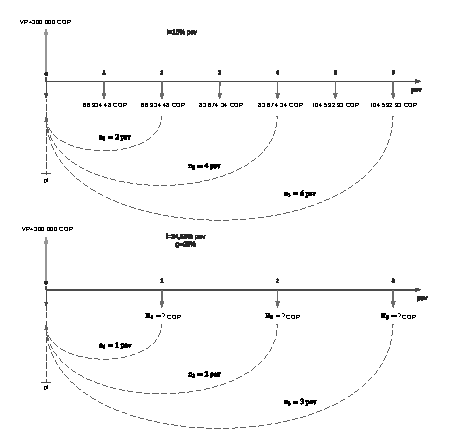
\includegraphics[trim=-78 -5 -78 -5,width=17cm]{7_Capitulo/img/ejemplos/8/8_3.pdf} } \\ \hline
			%%%%% INICIO FLUJO DE CAJA
			\rowcolor[HTML]{FFB183}
			\hline
			\multicolumn{1}{|c|}{\cellcolor[HTML]{FFB183}\textbf{4. Declaración de fórmulas}} \\ \hline
			%%%%%%%%%%%%% FIN INSERCIÓN DE IMAGEN
			%%%%% FIN FLUJO DE CAJA

			\multicolumn{1}{|c|}{ $VP = \frac{R( (1 + g)^{n} (1+i)^{-n} - 1)}{g-i} $ Valor presente gradiente geométrico } \\ \hline
			
			%%%%%% INICIO DESARROLLO MATEMÁTICO
			\rowcolor[HTML]{FFB183}
			\hline
			%%%%%%%%%% INICIO TÍTULO
			\multicolumn{1}{|c|}{\cellcolor[HTML]{FFB183}\textbf{5. Desarrollo matemático}} \\ \hline
			%%%%%%%%%% FIN TÍTULO
			%%%%%%%%%% INICIO MATEMÁTICAS
			\multicolumn{1}{|c|}{ $300{.}000 \; \text{COP} = \frac{R_{1}( (1 + 0{.}25)^{3} (1+0{.}3456)^{-3} - 1)}{0{.}25-0{.}3456} $ } \\ 
			\multicolumn{1}{|c|}{ $R_{1} = 225{.}920{,}73 \; \text{COP} $ } \\ \hline

			%%%%%%%%%% FIN MATEMÁTICAS
			%%%%%% FIN DESARROLLO MATEMÁTICO
			%%%%%% INICIO RESPUESTA
			\rowcolor[HTML]{FFB183}
			\hline
			%%%%%%%%%% INICIO TÍTULO
			\multicolumn{1}{|c|}{\cellcolor[HTML]{FFB183}\textbf{6. Respuesta}} \\ \hline
			%%%%%%%%%% FIN TÍTULO
			%%%%%%%%%% INICIO RESPUESTA MATEMÁTICA
			\multicolumn{1}{|c|}{ 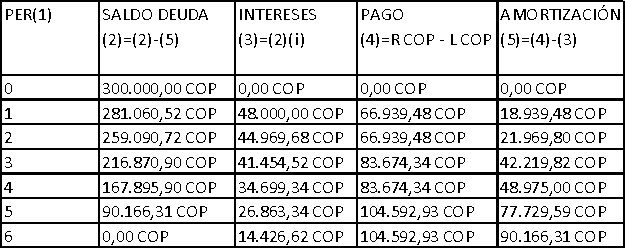
\includegraphics[trim=-78 -5 -78 -5]{7_Capitulo/img/ejemplos/8/8_3_3.pdf} } \\ \hline
		\end{longtable}
	\end{center}
%%%%%%%%%%%%%%%%%%%%%%%%%%FIN EJERCICIO 8c %%%%%%%%%%%%%%%%%%%%%%%%%%%
